\subsection{トポロジ}
グループは,ある数のセンサノードから構成される.グループ化のトポロジは,グループ内ではGMノードにGLノードが接続しGLノードとGWノードが接続するスター型トポロジとなる.

\begin{figure}[]
    \begin{center}
    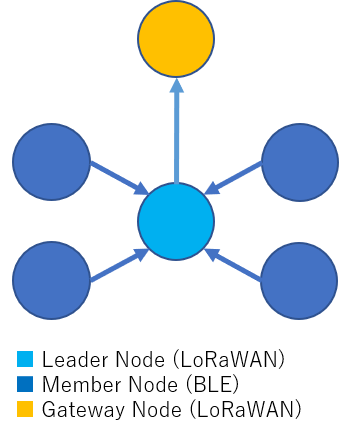
\includegraphics[width=5cm]{figures/グループ化のトポロジ.png}
    \caption{グループ化のトポロジ}
    \label{fig:group_topology}
    \end{center}
\end{figure}